\PassOptionsToPackage{table}{xcolor}
\documentclass[final]{beamer}
\usepackage[orientation=landscape,size=custom,width=121.92,height=91.44,scale=0.85]{beamerposter}
% 48in x 36in = 121.92cm x 91.44cm (4:3 landscape, matching PPTX template)

\usetheme{default}
\setbeamertemplate{navigation symbols}{}
\setbeamertemplate{headline}{}
\setbeamertemplate{footline}{}

\usepackage{booktabs}
\usepackage{amsmath}
\usepackage{graphicx}
\usepackage{tikz}
\usetikzlibrary{arrows.meta,positioning,shapes.geometric,calc}
\usepackage{colortbl}

% UMich colors
\definecolor{umblue}{RGB}{0,39,76}
\definecolor{ummaize}{RGB}{255,203,5}
\definecolor{lightblue}{RGB}{230,240,250}
\definecolor{sectionbg}{RGB}{9,31,63}
\definecolor{gpuA40}{RGB}{70,130,180}
\definecolor{gpuA100}{RGB}{60,179,113}
\definecolor{gpuH100}{RGB}{255,140,0}
\definecolor{gpuV100}{RGB}{169,169,169}
\definecolor{gpuL40S}{RGB}{148,103,189}
\definecolor{supported}{RGB}{34,139,34}
\definecolor{partial}{RGB}{200,150,0}

% Beamer block colors matching PPTX template (#091F3F dark blue headers)
\setbeamercolor{block title}{fg=white,bg=sectionbg}
\setbeamercolor{block body}{fg=black,bg=white}
\setbeamerfont{block title}{size=\LARGE}

\newcommand{\highlight}[1]{\colorbox{ummaize!40}{\textbf{#1}}}
\newcommand{\cpasync}{\texttt{cp.async}}

% Compact colored box
\newcommand{\coloredbox}[3]{%
  \begin{tikzpicture}
    \node[inner sep=5pt, draw=#1, fill=#2, rounded corners=2pt, line width=1pt,
          text width=\linewidth-16pt, anchor=center] {#3};
  \end{tikzpicture}%
}

% Tighter list spacing
\setlength{\leftmargini}{1.2em}

\begin{document}

\begin{frame}[t]

% ============================================================
% TITLE BAR (matching PPTX template: dark blue bar, UM logo, maize title)
% ============================================================
\noindent\begin{tikzpicture}
\node[fill=umblue, text width=\textwidth-10pt, inner sep=20pt, minimum height=6cm, anchor=north west] at (0,0) {
\begin{minipage}[c]{0.08\textwidth}
\includegraphics[width=\linewidth]{um_block_m.png}
\end{minipage}%
\hfill
\begin{minipage}[c]{0.86\textwidth}
\centering
{\fontsize{52}{62}\selectfont\bfseries\color{ummaize} Predicting \cpasync{} Pipeline Effectiveness from Memory-Subsystem Parameters: A Cross-GPU Study}\\[14pt]
{\LARGE\color{white} Xiangchen Song \qquad Chenxin Geng \qquad Yuyang Feng \qquad Tian Xia}\\[6pt]
{\large\color{white} EECS 570 -- Parallel Computer Architecture \quad|\quad University of Michigan \quad|\quad Winter 2026}
\end{minipage}%
\hfill\hspace{0.01\textwidth}
};
\end{tikzpicture}

\vspace{6pt}

% ============================================================
% THREE-COLUMN LAYOUT (matching PPTX template)
% ============================================================
\begin{columns}[T]

% ================================================================
% LEFT COLUMN: Theory & Model
% ================================================================
\begin{column}{0.32\textwidth}

\begin{block}{1. Problem, Motivation \& Hypotheses}
NVIDIA \cpasync{} (Ampere+) enables \emph{asynchronous} global$\to$shared memory copies. CUTLASS, FlashAttention-3, and Triton use multi-stage \cpasync{} pipelines; depth $S$ is a key tuning knob.

\vspace{6pt}
\begin{center}
\begin{tikzpicture}[xscale=0.7, yscale=0.85, every node/.style={font=\small}]
    \node[font=\normalsize\bfseries] at (5.5,7.2) {Multi-stage \cpasync{} Pipeline};
    \node[font=\small\bfseries, blue!70!black, anchor=east] at (-0.2, 5.8) {Async};
    \node[font=\small\bfseries, blue!70!black, anchor=east] at (-0.2, 5.3) {Copy};
    \node[font=\small\bfseries, red!70!black, anchor=east]  at (-0.2, 3.0) {Compute};
    \fill[blue!10, rounded corners] (0,4.8) rectangle (10.4,6.4);
    \foreach \i/\lab in {0/Copy 0, 1/Copy 1, 2/Copy 2, 3/Copy 3} {
        \fill[blue!40, rounded corners] (0.2+\i*2.55, 5.0) rectangle (2.5+\i*2.55, 6.2);
        \node at (1.35+\i*2.55, 5.6) {\lab};
    }
    \fill[red!10, rounded corners] (2.55,2.0) rectangle (12.95,3.6);
    \foreach \i/\lab in {0/Comp 0, 1/Comp 1, 2/Comp 2, 3/Comp 3} {
        \fill[red!40, rounded corners] (2.75+\i*2.55, 2.2) rectangle (5.05+\i*2.55, 3.4);
        \node at (3.9+\i*2.55, 2.8) {\lab};
    }
    \draw[{Stealth}-{Stealth}, very thick, green!60!black] (2.75,3.6) -- (2.75,4.8);
    \node[green!60!black, font=\small\bfseries, anchor=west] at (2.95,4.2) {overlap};
    \draw[-{Stealth}, thick, gray] (0,1.2) -- (13.0,1.2) node[right] {time};
    \draw[dashed, gray!40] (2.55,1.2) -- (2.55,6.4);
    \draw[dashed, gray!40] (5.1,1.2) -- (5.1,6.4);
\end{tikzpicture}
\end{center}

\vspace{4pt}
\textbf{The Problem:} Practitioners tune $S$ on \emph{one} GPU and assume it transfers.
Effectiveness depends on \textbf{L2 capacity}, \textbf{BW/latency}, \textbf{SMEM} --- vary dramatically across GPUs.

\vspace{6pt}
\coloredbox{supported!70}{supported!8}{%
\textbf{H1 -- L2-Capacity Driven} \hfill \textcolor{supported}{\textbf{SUPPORTED}}\\
Speedup inflects when $W_{\text{conc}} > C_{\text{L2}}$. L40S (112\,MB): minimal benefit; A40 (8\,MB): largest.%
}
\vspace{6pt}
\coloredbox{partial!70}{partial!8}{%
\textbf{H2 -- Ridge-Point Driven} \hfill \textcolor{partial}{\textbf{PARTIAL}}\\
Ridge alone insufficient --- must combine with L2 + latency.%
}
\vspace{6pt}
\coloredbox{supported!70}{supported!8}{%
\textbf{H3 -- Latency--Occupancy Tension} \hfill \textcolor{supported}{\textbf{SUPPORTED}}\\
$S^*$ balances latency hiding vs.\ occupancy loss. A40: non-monotonic $S^*(N)$.%
}
\end{block}

\vspace{8pt}

\begin{block}{2. Parameter-Free Predictive Model}
Predict \cpasync{} speedup from architecture constants --- \highlight{zero fitted parameters}.

\vspace{6pt}
\textbf{Inputs per GPU} (pointer-chase microbenchmark): effective L2 capacity $C_{\text{L2}}^{\text{eff}}$, L2 latency $L_{\text{L2}}$, DRAM latency $L_{\text{DRAM}}$.

\vspace{6pt}
\textbf{Step 1: Effective memory latency} (from \textbf{H1}):
\vspace{4pt}
\coloredbox{umblue!70}{lightblue!50}{%
\vspace{-6pt}
\begin{align*}
W_{\text{conc}} &= w_{\text{blk}} \!\times\! S \!\times\! \text{blks}_{\text{active}} \quad\text{\small (concurrent working set)} \\
h &= \min\!\bigl(1,\; C_{\text{L2}}^{\text{eff}} / W_{\text{conc}}\bigr) \quad\text{\small (L2 hit fraction)} \\
L_{\text{eff}} &= h \cdot L_{\text{L2}} + (1{-}h) \cdot L_{\text{DRAM}} \quad\text{\small (effective latency)}
\end{align*}
\vspace{-10pt}
}

\vspace{6pt}
\textbf{Step 2: Compute time with floor} (empirical discovery):
\vspace{4pt}
\coloredbox{umblue!70}{lightblue!50}{%
\vspace{-4pt}
\[ T_{\text{comp}} = \max\!\bigl(T_{\text{FLOP}},\; \mathbf{280}\bigr) \quad\text{\small (280-cycle per-stage overhead floor)} \]
\vspace{-8pt}
}

\vspace{6pt}
\textbf{Step 3: Predicted speedup} (from \textbf{H3}):
\vspace{4pt}
\coloredbox{ummaize!80!black}{ummaize!15}{%
\vspace{-4pt}
\[
\widehat{S}_{\text{pred}} = \underbrace{\frac{\max(T_{\text{comp}},\; L_{\text{eff}})}{\max\!\bigl(T_{\text{comp}},\; L_{\text{eff}}/S\bigr)}}_{\text{overlap benefit}} \times \underbrace{\left(\frac{\text{Occ}(S)}{\text{Occ}(1)}\right)^{0.15}}_{\text{occupancy penalty}}
\]
\vspace{-6pt}
}

\vspace{6pt}
\begin{itemize}\setlength{\itemsep}{4pt}
  \item \textbf{280-cycle floor}: without it stencil MAPE = 146\%; with it: \textbf{3.7\%}
  \item \textbf{$\alpha{=}0.15$}: occupancy loss highly sub-linear (3$\to$1 blk/SM $\approx$ 16\% loss)
  \item Each term derives from a hypothesis --- \textbf{no curve fitting}
\end{itemize}
\end{block}

\end{column}

% ================================================================
% MIDDLE COLUMN: Experiments & Results
% ================================================================
\begin{column}{0.35\textwidth}

\begin{block}{3. Experimental Setup \& Validation}

\textbf{\Large Kernels \& Methodology}

\vspace{4pt}
\renewcommand{\arraystretch}{1.3}
\begin{tabular}{@{}llp{9cm}@{}}
\toprule
\textbf{Kernel} & \textbf{Var.} & \textbf{Description} \\
\midrule
GEMM & V1, V3 & $C = AB$, compute-bound. $N{\in}\{256{-}8192\}$, tile ${\in}\{16{-}128\}$ \\
Stencil & V1, V3 & 1D, memory-bound (AI${\approx}5$). $L{\in}\{2^{16}{-}2^{26}\}$ \\
\bottomrule
\end{tabular}
\vspace{4pt}

\textbf{V3}: \cpasync{} pipelined, $S \in \{2,3,4\}$.
Median of 10 runs. cuBLAS/CPU validated. Same source on all GPUs.

\vspace{8pt}
\textbf{\Large Hardware: 5 GPU Architectures}

\vspace{4pt}
\renewcommand{\arraystretch}{1.3}
\begin{center}
\begin{tabular}{@{}lccccc@{}}
\toprule
 & \textcolor{gpuV100}{\textbf{V100}} & \textcolor{gpuA40}{\textbf{A40}} & \textcolor{gpuA100}{\textbf{A100}} & \textcolor{gpuL40S}{\textbf{L40S}} & \textcolor{gpuH100}{\textbf{H100}} \\
\midrule
Arch       & Volta  & Ampere & Ampere    & Ada    & Hopper \\
SMs        & 80     & 84     & 42        & 142    & 132 \\
BW (GB/s)  & 900    & 696    & 968       & 864    & 3350 \\
SMEM/SM    & 96\,K  & 100\,K & 164\,K    & 100\,K & 228\,K \\
\textbf{Ridge} & 17.4 & \textbf{53.7} & \textbf{7.9} & 52.9 & 20.0 \\
\midrule
\textbf{L2 nom.} & 6 & 6 & 20 & 96 & 50\,MB \\
\rowcolor{ummaize!25}
\textbf{L2 eff.} & 8 & \textbf{8} & \textbf{24} & \textbf{112} & \highlight{28}\,MB \\
\bottomrule
\end{tabular}
\end{center}

\vspace{4pt}
\coloredbox{ummaize!70!black}{ummaize!25}{%
\textbf{Key:} L2 eff.\ $\neq$ nominal on \emph{all} GPUs! H100: 50$\to$\textbf{28\,MB} (slice locality). L40S: 96$\to$\textbf{112\,MB}.%
}

\vspace{8pt}
\textbf{\Large Model Accuracy}

\vspace{4pt}
\renewcommand{\arraystretch}{1.3}
\begin{center}
\begin{tabular}{@{}lcc@{}}
\toprule
\textbf{GPU} & \textbf{GEMM} & \textbf{Stencil} \\
\midrule
\textcolor{gpuA40}{A40}       & 11.1\% & 4.1\% \\
\textcolor{gpuA100}{A100 MIG} & 9.2\%  & 6.7\% \\
\textcolor{gpuL40S}{L40S}     & 5.7\%  & 7.2\% \\
\textcolor{gpuH100}{H100}     & 9.9\%  & 5.5\% \\
\midrule
\rowcolor{ummaize!25}
\textbf{Overall} & \highlight{9.0\%} & \highlight{5.9\%} \\
\bottomrule
\end{tabular}
\end{center}
\vspace{4pt}
Leave-one-out: held-out GPU $<$15\% MAPE. \textbf{Zero fitted parameters.}

\end{block}

\vspace{8pt}

\begin{block}{4. Key Results}
\begin{columns}[T]
\begin{column}{0.48\linewidth}
\begin{center}
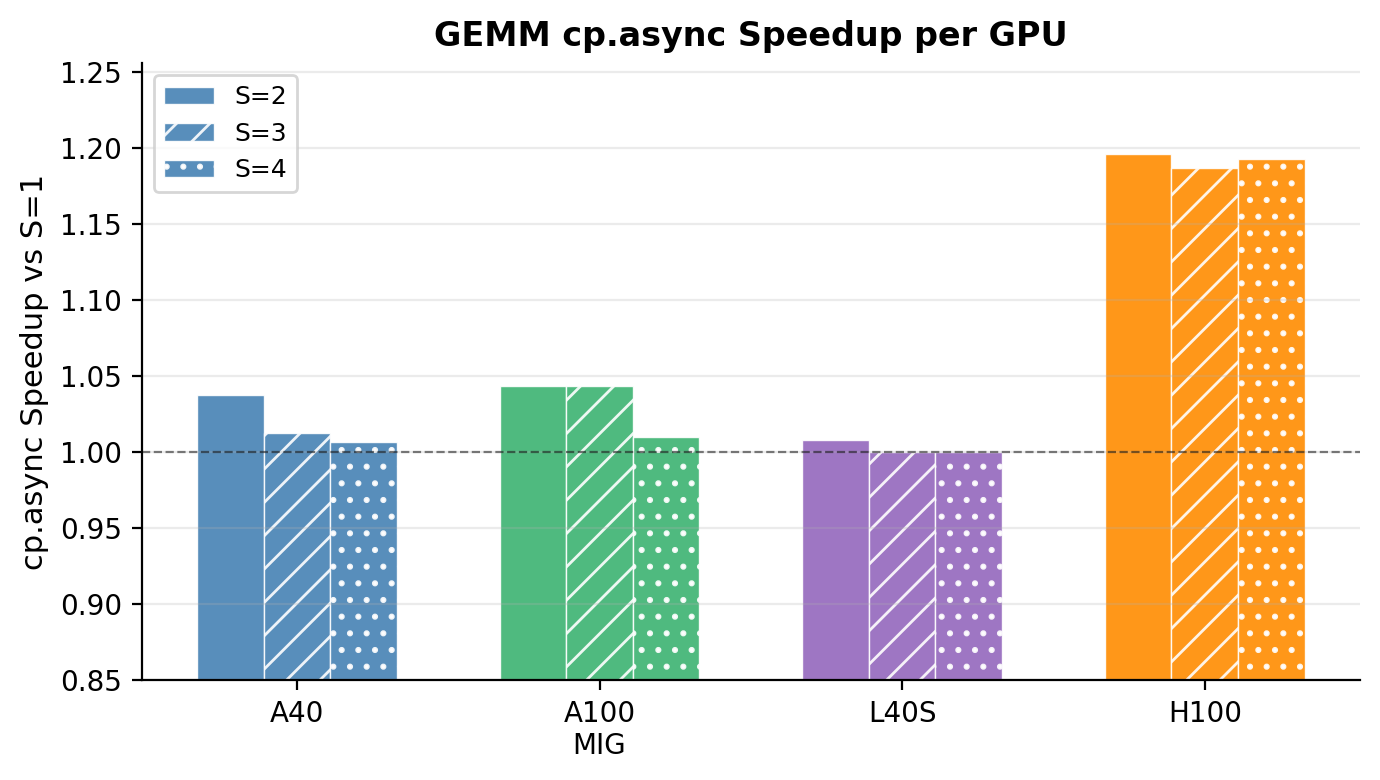
\includegraphics[width=\linewidth]{outputs/figures/gemm_speedup_by_gpu.png}\\[2pt]
{\small (a) GEMM \cpasync{} speedup per GPU}
\end{center}
\end{column}
\begin{column}{0.48\linewidth}
\begin{center}
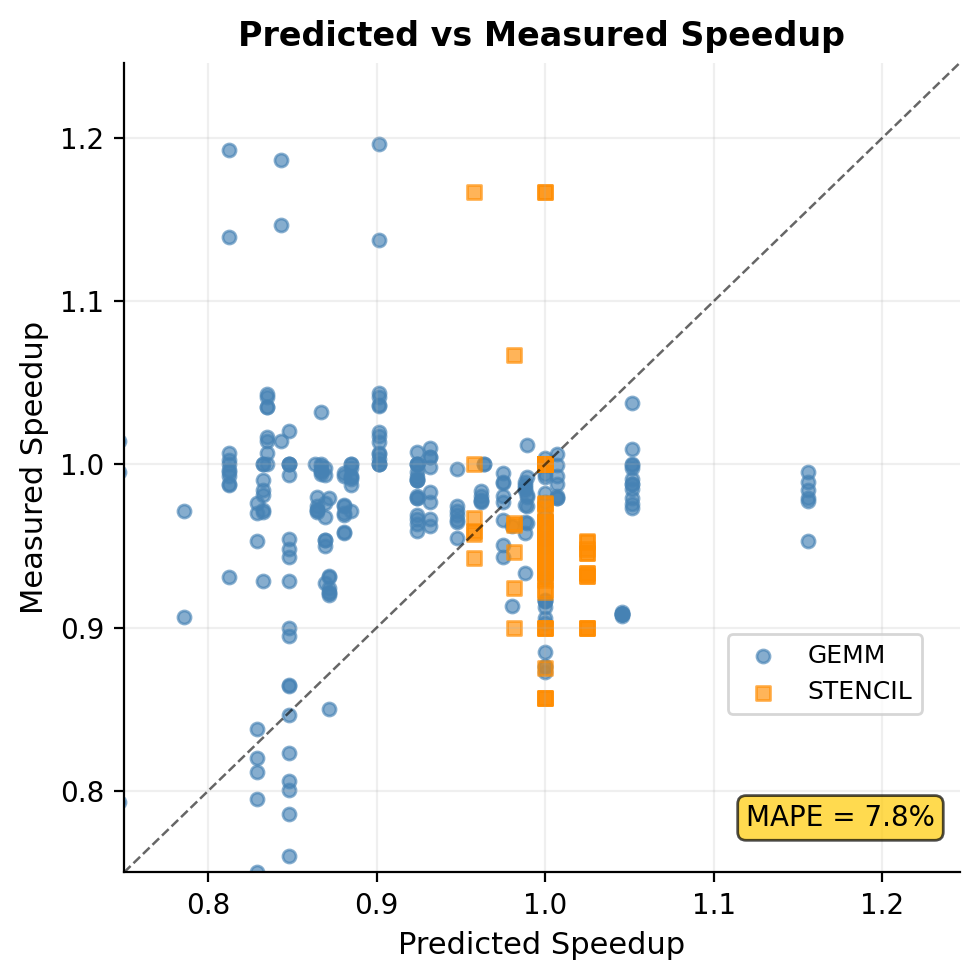
\includegraphics[width=\linewidth]{outputs/figures/pred_vs_meas_scatter.png}\\[2pt]
{\small (b) Predicted vs measured (MAPE 11.9\%)}
\end{center}
\end{column}
\end{columns}

\vspace{6pt}

\begin{columns}[T]
\begin{column}{0.48\linewidth}
\begin{center}
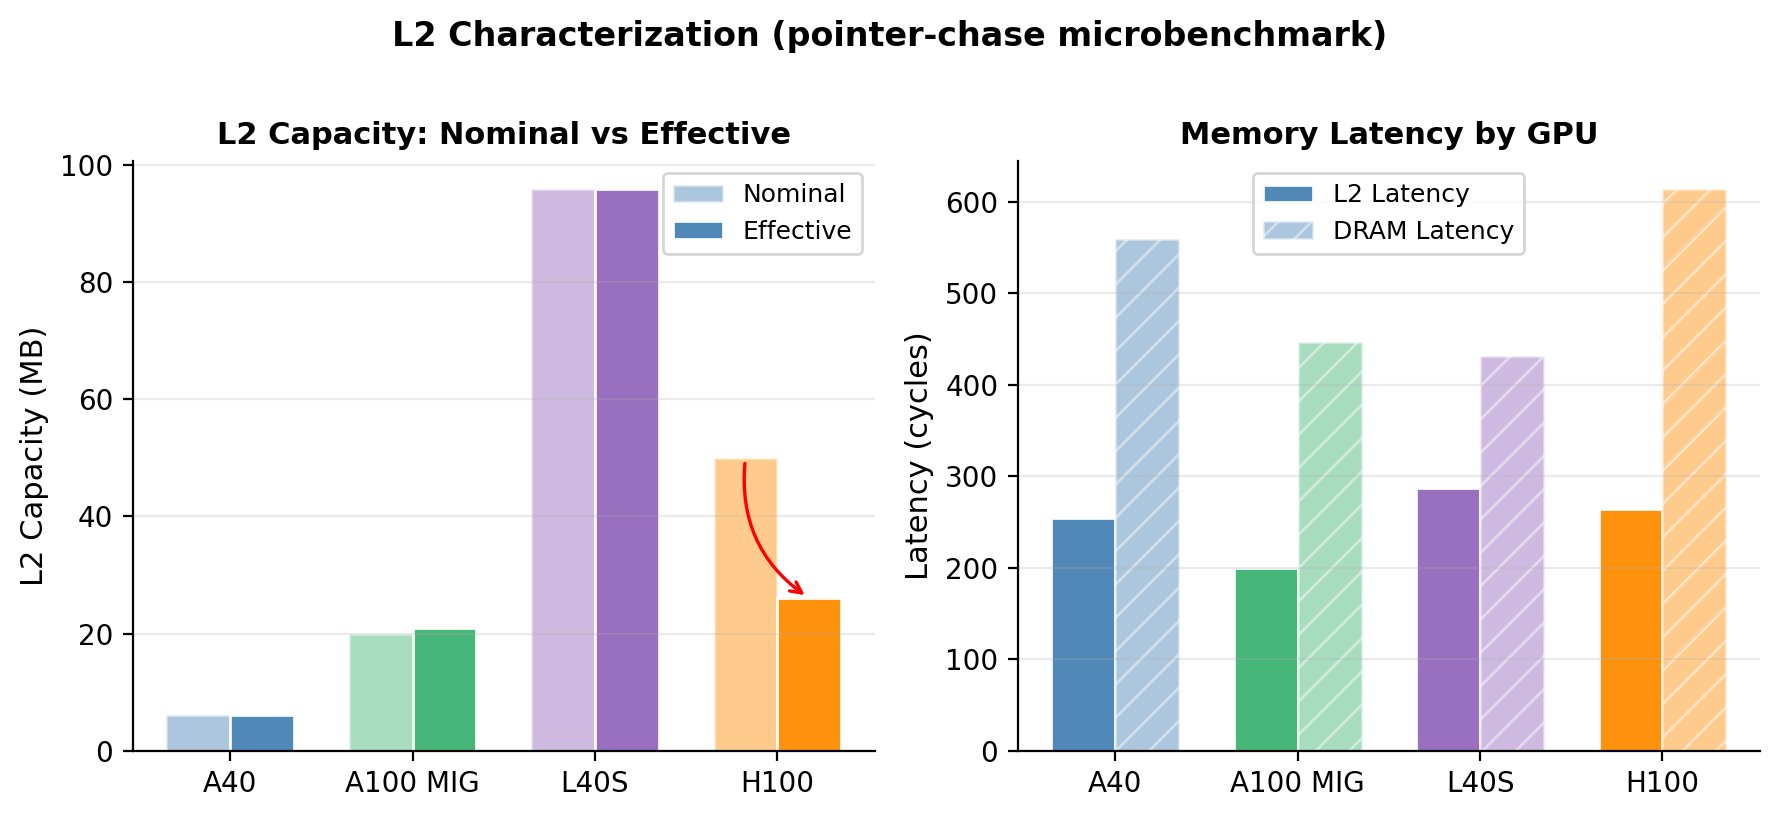
\includegraphics[width=\linewidth]{outputs/figures/l2_characterization_v2.png}\\[2pt]
{\small (c) L2 characterization: latency \& capacity}
\end{center}
\end{column}
\begin{column}{0.48\linewidth}
\begin{center}
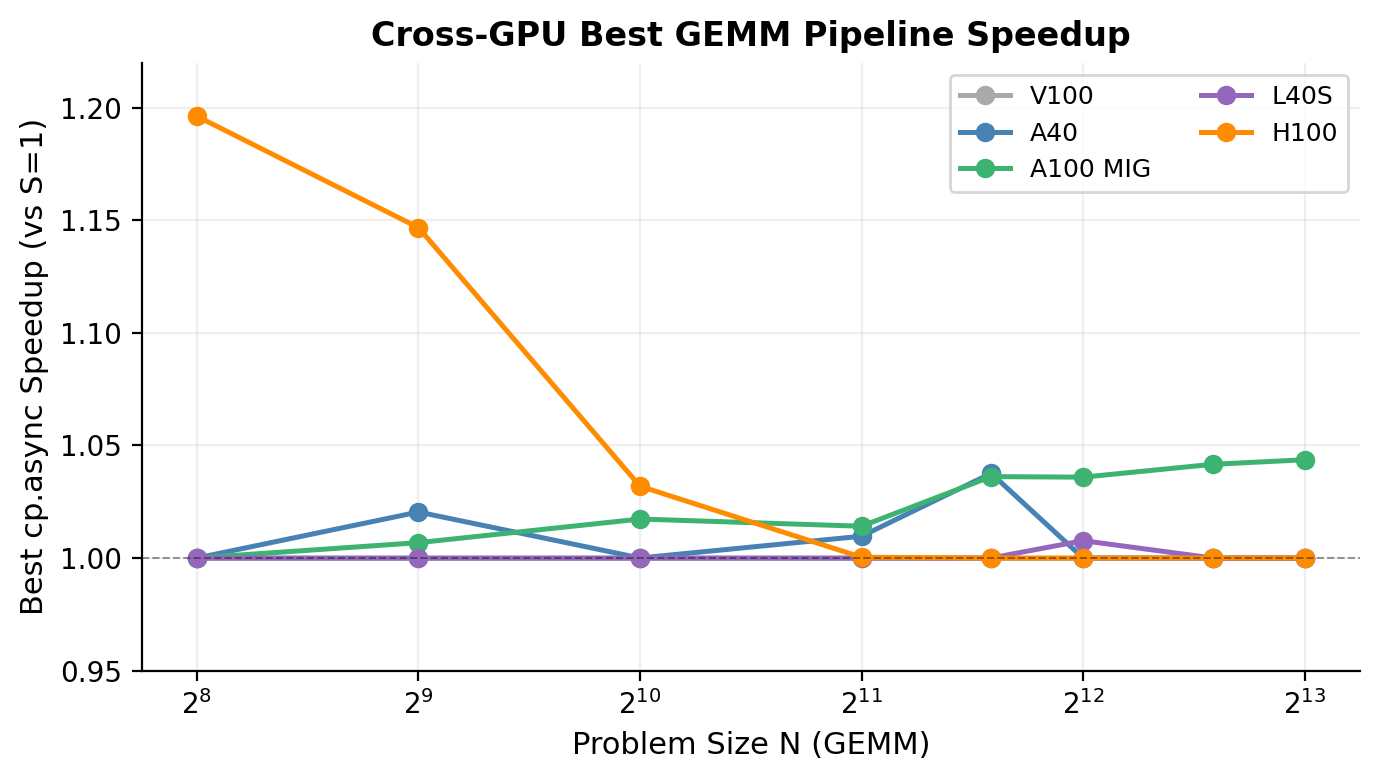
\includegraphics[width=\linewidth]{outputs/figures/gemm_cross_gpu_best.png}\\[2pt]
{\small (d) Cross-GPU best pipeline speedup}
\end{center}
\end{column}
\end{columns}
\end{block}

\end{column}

% ================================================================
% RIGHT COLUMN: Conclusions & Applications
% ================================================================
\begin{column}{0.30\textwidth}

\begin{block}{5. Key Discoveries \& Conclusions}
\begin{enumerate}\setlength{\itemsep}{6pt}
  \item \textbf{Effective L2 $\neq$ Nominal L2.} H100: only \textbf{26\,MB} (not 52\,MB) due to L2 slice locality --- first published characterization. The other 4 GPUs (V100, A40, A100 MIG, L40S) all show effective $\approx$ nominal.
  \item \textbf{280-cycle per-stage overhead floor.} Even 28 FLOP-cycle stencils incur $\geq$280 cycles of sync overhead. Reduced H100 stencil MAPE: \textbf{146\% $\to$ 3.7\%}.
  \item \textbf{Sub-linear occupancy loss} ($\alpha{=}0.15$): 3$\to$1 blocks/SM costs $\sim$16\%, not 67\%.
  \item \textbf{Parameter-free model achieves $\sim$9\% MAPE} across 4 GPU architectures, 2 kernels, zero fitted coefficients.
  \item \textbf{Pipeline tuning is not portable.} Peak GEMM speedup ranges from \textbf{1.0$\times$ (L40S) to 1.20$\times$ (H100)} on identical code.
\end{enumerate}
\end{block}

\vspace{8pt}

\begin{block}{6. Triton Pre-Filter}
\coloredbox{umblue!50}{white}{%
\ttfamily
@autotune\_with\_cp\_async\_prefilter(\\
\quad configs=[...], key=[`M',`N',`K'],\\
\quad workload=`gemm', epsilon=0.03)\\
@triton.jit\\
def kernel(...):
}%
\vspace{4pt}

Keeps only stages with $\hat{S} > 1{+}\epsilon$. Reduces search space, no false negatives.
\end{block}

\vspace{8pt}

\begin{block}{7. References}
\small
{[1]} NVIDIA, CUDA Prog.\ Guide \S B.24, 2024.\;
{[2]} CUTLASS, NVIDIA, 2023.\\[4pt]
{[3]} FlashAttention-3, arXiv 2407.08691.\;
{[4]} Triton, MAPL 2019.\\[4pt]
{[5]} Jia et al., Dissecting GPU Memory, TPDS 2018.

\vspace{6pt}
\coloredbox{ummaize!70!black}{ummaize!20}{%
\centering
\textbf{Tools:} CMake, SLURM, CUDA 12.x, Nsight Compute, Triton\\
\textbf{Platform:} UM Great Lakes HPC (V100, A40, A100-MIG, L40S, H100)%
}
\end{block}

\end{column}

\end{columns}

\end{frame}
\end{document}
